\documentclass{standalone}

\usepackage{setspace}
\usepackage{times}
\usepackage{amsmath}
\usepackage{amssymb}
\usepackage{xparse}
\usepackage{ifthen}

\usepackage[dvipsnames]{xcolor}
\usepackage{tikz}
\usetikzlibrary{arrows,calc,patterns,patterns.meta}
\pgfdeclarelayer{background}
\pgfdeclarelayer{foreground}
\pgfsetlayers{background,main,foreground}

\usepackage{pgfplots}
\pgfplotsset{compat=1.15}

\renewcommand{\seriesdefault}{\bfdefault}
\renewcommand{\familydefault}{\sfdefault}

\begin{document}
    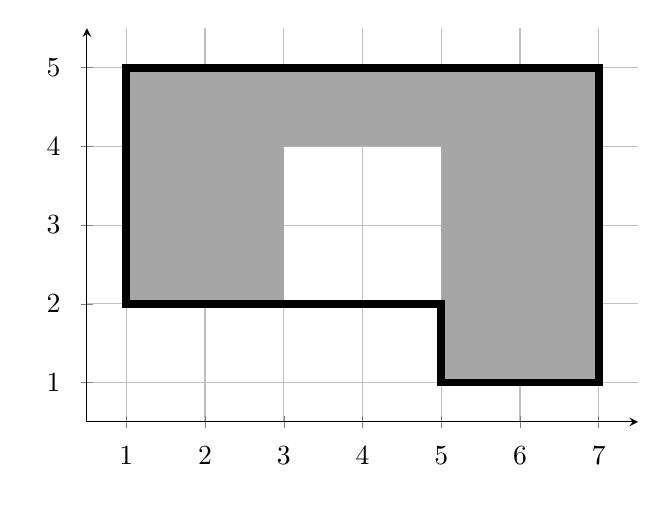
\begin{tikzpicture}[x=1cm,y=1cm,every node/.style={circle,inner sep=0pt,line width=1pt, minimum size = 0.66cm}]
        \begin{axis}[
            x=1.0cm,y=1.0cm,
            axis lines=middle,
            ymajorgrids=true,
            xmajorgrids=true,
            xmin=0.5,
            xmax=7.5,
            ymin=0.5,
            ymax=5.5,
            xtick={1.0,...,7.0},
            ytick={1.0,...,5.0},]  
			\fill[fill=gray!70!white] (1,2) -- (3,2) -- (3,4) -- (5,4) -- (5,1) -- (7,1) -- (7,5) -- (1,5) -- cycle;
			\draw[draw=black,line width=0.1cm] (7,5) -- (1,5) -- (1,2) -- (5,2) -- (5,1) -- (7,1) -- cycle;
        \end{axis}
    \end{tikzpicture}
\end{document} 
